\documentclass{article}
\usepackage[margin=1in]{geometry}
\usepackage{setspace, fancyhdr, hyperref, xcolor, tikz}
\usetikzlibrary{positioning, intersections, calc, arrows}
\usepackage[square,numbers]{natbib}
\bibliographystyle{abbrvnat}

\newcommand{\thetitle}{Symbolic Manipulation and Computation in the Same Graph}
 
\pagestyle{fancy}
\fancyhf{}
\rhead{\thetitle}
\lhead{Darius Barbano}
\rfoot{Page \thepage}
\doublespacing



\author{Darius Barbano}
\title{\thetitle}
\date{}

\begin{document}

\maketitle
\newpage
\tableofcontents
\newpage

\begin{abstract}
    General artificial intelligence refers to machine intelligence than performs a task as successfully as a human does. A fundamental difference between human neural network and current machine neural networks is that only human networks combine symbolic reasoning with computation. Here we show how a graph can \ldots
\end{abstract}
\newpage


\section{Background}

    \begin{enumerate}
        \item What is symbolic computation?
        
        A symbolic computation is a calculation performed with symbolic representations of values and operations. A simple example would be the expression $(x + 1)(x - 1)$ which would evaluate to $x^2 - 1$, rather than to some numerical result.

        \item What is calculation?
        
        A calculation is a process by which one or more inputs is transformed into one or more results. One may calculate that the product of 5 and 4 is 20.
        
        \item What is meant by a computational class? \textcolor{red}{- do you mean complexity class?}
        
        
    \end{enumerate}
    
     Code for each subsection of this document can be found at \href{https://github.com/DariusBxsci/NeuralNetworkResearch/tree/master/NeuralNets}{NeuralNetworkResearch}. 


\section{Methods}

\subsection{Network Construction}

 Figure \ref{fig:sig-neuron} illustrates a neuron that receives three ordered inputs. 
 
 \begin{figure}[h]
 \centering
 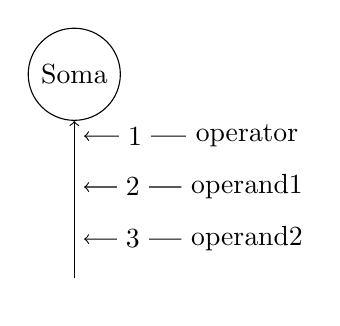
\begin{tikzpicture}

 
    \node[circle, draw=black] (soma) {Soma};
    \node[below= 2cm of soma] (dendrite) {};
    
    \begin{scope}[node distance=1mm and 10mm]
    \node[below right = of soma] (operator) {operator};
    \node[below = of operator] (operand1) {operand1};
    \node[below = of operand1] (operand2) {operand2};
    \end{scope}
    
    
    \draw[->] (dendrite) -> (soma);
    
    
    %nodes along dendrite
    \node (operator'dendrite) at (intersection of operator--soma|-operator and dendrite--soma){};
    
    \node (operand1'dendrite) at (intersection of operand1--soma|-operand1 and dendrite--soma){};
    
    \node (operand2'dendrite) at (intersection of operand2--soma|-operand2 and dendrite--soma){};
    
    
    \draw[->] (operator) -- (operator'dendrite) node[midway, fill=white] {1};
    \draw[->] (operand1) -- (operand1'dendrite) node[midway, fill=white] {2};
    \draw[->] (operand2) -- (operand2'dendrite) node[midway, fill=white] {3};
    
 \end{tikzpicture}
 \caption{Single neuron receiving ordered intputs. \label{fig:sig-neuron}}
\end{figure}
 

\section{Results}

\section{Conclusions}

\bibliography{references}

\end{document}